\subsection{The \bap Intermediate Language}


\begin{table}
\centering
\begin{tabular}{lll}
  \emphkind{program}&::=&
        \emphkind{stmt}*\\

  \emphkind{stmt}&::=&  
         \emphkind{var} := \emphkind{exp}
     $|$ {\tt jmp}(\emphkind{exp})
     $|$ {\tt cjmp}(\emphkind{exp},\emphkind{exp},\emphkind{exp})\\
     &&$|$ {\tt halt}(\emphkind{exp})
     $|$ {\tt assert}(\emphkind{exp})
     $|$ {\tt label} \emphkind{label\_kind}
     $|$ {\tt special}(string)\\

  \emphkind{exp}&::=& 
         {\tt load}(\emphkind{exp}, \emphkind{exp}, \emphkind{exp},
         \emphkind{$\tau_{\text{reg}}$})
        $|$ {\tt store}(\emphkind{exp}, \emphkind{exp},
        \emphkind{exp},\emphkind{exp},$\tau_{\text{reg}}$ )
     $|$ \emphkind{exp} $\Diamond_b$ \emphkind{exp}
     \\
     & & 
     $|$ $\Diamond_u$ \emphkind{exp}
     $|$ \emphkind{var}
     $|$ {\tt lab}(string)
     $|$ \emphkind{integer}
     $|$ {\tt
       cast}(\emphkind{cast\_kind},$\tau_{\text{reg}}$,\emphkind{exp})
\\
     & & $|$ {\tt let} \emphkind{var} {\tt =} \emphkind{exp} {\tt in} \emphkind{exp}
    
     $|$ {\tt unknown}(string, $\tau$)
     $|$ {\tt name}(\emphkind{exp})
     \\

  \emphkind{label\_kind}&::=&  \emphkind{integer} $|$ string \\
     
  \emphkind{cast\_kind}&::=&  
     {\tt unsigned}
     $|$ {\tt signed}
     $|$ {\tt high} 
     $|$ {\tt low}\\

%   \emphkind{decl}&::=& 
%          {\tt var} \emphkind{var}\\


  \emphkind{var}&::=& 
         (string, id$_v$, $\tau$)\\

  $\Diamond_b$&::=&
     $+ , - , * ,  /, /_s , \bmod , \bmod_s , \ll, \gg, \gg_a ,  \&,
        |, \xor, ==, !=, <, \leq , <_s, \leq_s$\\

  $\Diamond_u$&::=& $-$ (unary minus), $\sim$ (bit-wise not)\\

  \emphkind{value}&::=&  \emphkind{integer}
       $|$ \emphkind{memory} 
       $|$ string
       $|$ $\perp$  \\

  \emphkind{integer}&::=&          $n$ (:$\tau_{\text{reg}})$ \\


  \emphkind{memory}&::=&
        \{ \emphkind{integer} $\rightarrow$ \emphkind{integer}, 
             \emphkind{integer} $\rightarrow$ \emphkind{integer},
             \ldots \} (:$\tau_{\text{mem}}$) \\

  \emphkind{$\tau$} &::=&
          \emphkind{$\tau_{\text{reg}}$} 
      $|$ \emphkind{$\tau_{\text{mem}}$}\\

  \emphkind{$\tau_{\text{mem}}$} &::=& {\tt mem\_t}($\tau_{\text{reg}}$)
  $|$ {\tt array\_t}($\tau_{\text{reg}}, \tau_{\text{reg}}$)\\\
  
  \emphkind{$\tau_{\text{ reg}}$}&::=&
         {\tt reg1\_t} 
      $|$ {\tt reg8\_t} 
      $|$ {\tt reg16\_t} 
      $|$ {\tt reg32\_t} 
      $|$ {\tt reg64\_t}\\



\end{tabular}
\caption{The Binary Intermediate Language. Note commas separte
  operators.}
\label{vine:syntax}
\end{table}



Table~\ref{tab:vine-il} shows the \bap intermediate language. A program
in the IL is a sequence of instructions (\emphkind{instr}).  In
Section~\ref{vine:opsemantics} we give the operational semantics of
the IL.  Here, we give an informal description of the IL. We also
discuss how assembly is lifted to the IL, and how the semantics of
assembly influenced the IL.

Instructions are similar to those found in a RISC-based
architecture. The advantage of providing relatively few instruction
types is that it simplifies many types of analysis. A typical program
analysis paradigm (e.g., data-flow analysis) is to visit each
instruction, then do a case analysis on the type of instruction. By
minimizing the number of instructions, we minimize the number of cases
that need to be analyzed.

The semantics of most instructions are relatively straight-forward and
unsurprising: we have assignments, conditional and unconditional
jumps, halting the program, program blocks which scope variables, {\tt
  assert}, which behaves like an assert statement in C.  A {\tt label}
denotes a labeled program location, and roughly corresponds to an
instruction address.  A {\tt special} instruction represents an
undefined state update to the program.  For example, an interrupt call
is lifted as a {\tt special}, with the kind indicating the interrupt
number.  The point of having {\tt special} is to indicate where an
analysis needs to provide additional information, e.g., replacing an
interrupt with an appropriate summary of the desired effects of
executing the interrupt.  Thus, the only purpose of {\tt special} is
to aide analysis: the actual operational semantics of {\tt special}
are undefined.


The semantics of expressions is straight-forward. We support the
standard binary and unary ops. A subscript $s$, such as $/_s$,
indicates an operation on signed numbers (because signed division is
handled differently than unsigned).  The $\gg_a$ corresponds to
arithmetic right shift.  The cast unary operators are used when
lifting from assembly to the IL. For example, in assembly the lower
8-bits of a register may be assigned to a 32-bit register. In this
case, we must cast to fill in whether the assignment sign-extends or
not.   We also introduce {\tt let} expressions, which essentially act
as side-effect free scoping that makes certain kinds of analysis
easier to express.  

There are three different types of variables in the IL: scalars,
memories, and arrays. Registers in assembly correspond to IL scalar
variables, e.g., the x86 {\tt eax} register correspond to the {\tt
  eax} register of type {\tt reg32\_t}.  One issue we must deal with
is a single register may have several names, with each name
corresponding to specific register bits. For example, in x86 the name
{\tt al} refers to the lower 8-bits of the {\tt eax} register, i.e.,
is a type of scalar aliasing.  When lifting assembly, we use the
canonical name for each register and replace names accessing specific
bits with the relevant operations. For example, a store into {\tt al}
in x86 is written as a store into the 8 lower bits of variable {\tt
  eax}.  The canonicalization is done to make analysis easier: in
\bap and unlike assembly, scalars never are aliased by another name.

The type of a memory variable includes the endianess and the index
type. For example on x86 we initially define one memory which the
whole program uses of type {\tt mem$_\text{little}$\_t:reg32\_t} since
x86 is little endian and indexes are 32-bit integers. Although on a
real machine there is only one memory, we allow for multiple memories
because it may aide program analysis.  For example, an analysis may
divide up memory into individual stack frames and the heap.

A memory access (either a load or store) is given by the tuple {\tt
  mem($v$, $e$, $\tau_{\text{reg}}$} where $v$ is the memory to
operate on, $e$ is the address (and thus should match the declared
address type for $v$), and $\tau_{\text{reg}}$ is the number of bytes
to access.  For example, loading a 32-bit word at location $c$ from
memory $m$ into register $r$ is written {\tt r:= mem($m$, $c$,
  reg32\_t)}.

An array of type {\tt array\_t[$i$]:$\tau$} denotes an array that
contains $i$ slots, each of which holds members of type $\tau$. We
also use {\tt mem} to denote an array access. Since array accesses
must be all of the same type, $\tau_{\text{reg}}$ in a {\tt mem}
statement is not needed. However, to keep things simple we did not
introduce a new expression type to denote array accesses.

\begin{figure}

\subfloat[t]{
\begin{minipage}{3.2in}
\begin{small}
\begin{tightcode}
1. $r_1$ := 0xaabbccdd;
2. $r_2$ := 0x1122;
// mov dword [$c$], $r_1$
3. mem($m$, $c$, reg32\_t) := $r_1$;
// mov word [$c+3$], $r_2$
4. mem($m$, $c+3$, reg16\_t) := $r_2$;
5. $r_1$ := mem($m$, $c$, reg32\_t);
\end{tightcode}
\end{small}
\end{minipage}
}
%\end{minipage}
%\begin{minipage}{3 in}
\subfloat[]{
\includegraphics[scale=.9]{fig/memvsarray-1}
\label{fig:beforeline4}
}
\subfloat[]{\label{fig:afterline4}}{
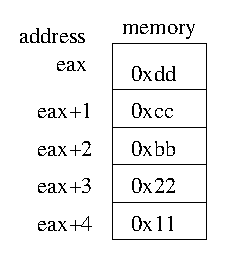
\includegraphics[scale=.9]{fig/memvsarray-2}
}
\end{minipage}
\caption{The \bap program on the left-hand side writes a 32-bit and
  16-bit value to memory $m$ at address $c$ and $c+3$. (a) shows the
  values in memory before executing line 4, and (b) shows memory after
  executing line 4. The value of $r_1$ after line 5 is 0x11bbccdd.}
\label{fig:broken-mems}
\end{figure}

A contiguous portion of memory can be modeled either as a memory
variable or an array.  However, most analysis benefit from modeling
memory as an array.  The reason is the array representation of memory
--- e.g., you give me an 32-bit number, I give you back an 8-bit value
--- reduces all memory access to the same type. Further, multiple
stores cannot overlap.  With memory, two stores may overlap. 

For example, in Figure~\ref{fig:broken-mems} the two memory store
operations have overlapping ranges.  Note that it is not uncommon to
find overlapping stores, e.g., arising from type-casting in C.  An
analysis of this program would have to keep track of the fact that the
writes on line 3 and 4 overlap.


In Section~\ref{sec:deend} we show how we convert memory accesses to
array accesses.  The conversion rewrites memory accesses to byte-level
accesses where each memory access denotes accessing a single cell.

% \subsection{The \bap Core Language}


% \begin{table}
% \centering
% \begin{tabular}{lll}
%   \emphkind{program}&::=&\emphkind{instr}*\\
%   \emphkind{instr}&::=&  
%   \emphkind{var} := \emphkind{exp} 
%   $|$ {\tt jmp} $e$
%   $|$ {\tt halt} $e$\\
%   \emphkind{exp}&::=& 
%   {\tt load}(\emphkind{var}, \emphkind{exp})
%   $|$ \emphkind{exp} $\Diamond_b$ \emphkind{exp} 
%   $|$ $\Diamond_u$ \emphkind{exp}
%   $|$ \emphkind{value} $|$ {\tt cast}(\emphkind{cast\_kind},
%   $\tau_{\text{reg}}$) \\
%   \emphkind{cast\_kind}&::=&  {\tt cast\_unsigned}
%   $|$ {\tt cast\_signed}
%   $|$ {\tt cast\_high} 
%   $|$ {\tt cast\_low}\\
%   \emphkind{var}&::=& string, id, $\tau$\\
%   \emphkind{$\tau_{\text{ reg}}$}&::=&{\tt reg1\_t} $|$ {\tt reg8\_t} $|$ {\tt reg16\_t} $|$
%   {\tt reg32\_t} $|$ {\tt reg64\_t}\\
%   \emphkind{$\tau$} &::=&\emphkind{$\tau_{\text{reg}}$} 
%   $|$ {\tt array\_t[}\emphkind{value}{\tt ]}:\emphkind{$\tau_{\text{reg}}$}\\
%   $\Diamond_b$&::=&$+,-,*, /, /_s , \bmod , \bmod_s , \ll, \gg, \gg_a ,  \&,
%   |, \xor, =, \neq, <, \leq , <_s, \leq_s$\\
%   $\Diamond_u$&::=&$\neg | !$  \\
%   \emphkind{value}&::=& integer:$\tau_{\text{reg}}$ $|$ $\bot$\\
% \end{tabular}
% \caption{The \bapcore Language. }
% \label{tab:vine-core-il}
% \end{table}


% The \bap language shown in Table~\ref{tab:vine-il} contains several
% elements that act as ``syntatic sugar'' --- they express commonly
% occuring patterns succiently, but they do not add expressive power to
% the language.  In Table~\ref{tab:vine-core-il} we show the core
% \bapcore language. The advantage of syntatic sugar
% present in \bap is that it makes writing analysis easier.  The
% advantage of defining \bap is that when we describe
% algorithms and formalize the semantics, we need only do it in terms of
% the smaller language.

% \begin{table}
%   \begin{tabular}{lp{2in}p{2in}}
%     \bap & \bapcore & Description\\
%     {\tt special} $s$ & {\tt assert}(0) & A {\tt special} statement
%     is not part of the operational semantics. Simply abort.\\
%     {\tt assert}($e$) & {\tt cjmp}($e$,
%     $\langle$next$\rangle$,$\langle$fail$\rangle$) \newline 
%     ...\newline
%     {\tt label} $\langle$fail$\rangle$: halt $\bot$
%     & When $e$ is true, execute the next statement. When $e$ is false,
%     jump to a code block that causes the machine to halt with  value
%     $\bot$, indicating abort. \\
%     {\tt cjmp}($e$, $e_t$, $e_f$) & 
%     $r_1$ := {\tt cast}({\tt signed}, $e$) $\& e_t$ \newline
%     $r_2$ :=  {\tt cast}({\tt signed}, $!e$) $\& e_f$ \newline
%     {\tt jmp}($r_1 | r_2$) & Foo
%   \end{tabular}
% \end{table}


% \bap can be reduce to \bapcore by:
% \begin{itemize}\squish
%   \item Descoping (with $\alpha$-varying as necessary) all blocks
%     ({\tt \{ instr* \}}) and {\tt let} expressions as necessary.
%   \item Replacing each derived form as shown in
%     Table~\ref{tab:derived}. Note that the rules are applied in order
%     to the whole program, resulting in a program free of {\tt assert},
%     {\tt special}, etc. 
    
% \end{itemize}
